\subsection{Motivation}
    \begin{frame}{Problem}
        As part of the COVID-19 vaccination campaing, on December 02
        2020, Mexican goverment anunciates a series of the ***
        vaccine deliveries by Pfizer-BioNtech.
        \begin{textblock*}{130mm}(1mm, 20mm)
        \only<1>{
            %\begin{bluebox}{Delivery schedule}
                \begin{center}
                    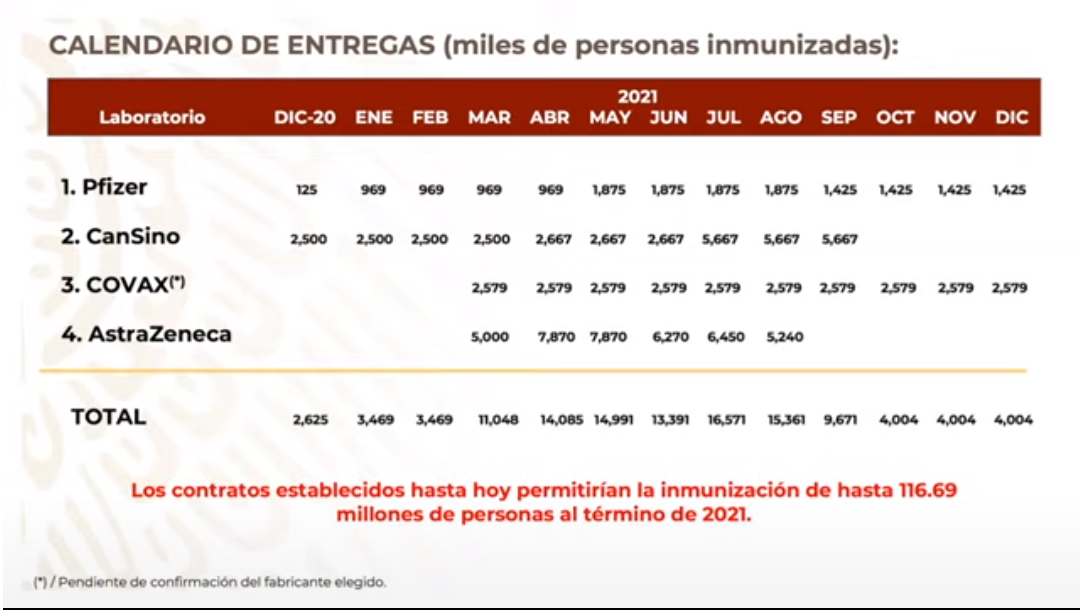
\includegraphics[%
                        width=\textwidth,
                        keepaspectratio=true]{screenshot.png}
                \end{center}
            %\end{bluebox}
        }
    \end{textblock*}
    \end{frame}
%
\begin{frame}{Argument}
    \begin{textblock*}{50mm}(10mm, 30.0mm)
            We argue that sufficiently large random fluctuations in
        deliveries\textemdash due to lags or the
        number of vaccines doses\textemdash convey significantly
        effects on the mitigation of
        symptomatic cases.
\end{textblock*}

    \begin{textblock*}{50mm}(70mm, 30.0mm)
    \begin{block}{Aims}
        We pursue quantifying the uncertainty due to time lags or amount
        delivery, and evaluates its implications.
    \end{block}
    \end{textblock*}
\end{frame}
%%%%
\subsection{Methodology}
    \begin{frame}{Methodology}
        Given a shipment of vaccines calendar, describe the stock management with
        backup protocol and quantify random fluctuations due to schedule or
        quantity. Then plug this dynamic with an ODE system that describes the
        disease and evaluates its response accordingly.
    \end{frame}
%
\begin{frame}{Vaccine Shipment Program}
    As part of the COVID-19 vaccination campaign, on December 02, 2020, the
    Mexican government annunciated a delivery plan of vaccines by Pfizer-BioNTech
    and other firms.
    \begin{textblock*}{130mm}(1mm, 20mm)
    \only<2>{
        %\begin{bluebox}{Delivery schedule}
            \begin{center}
                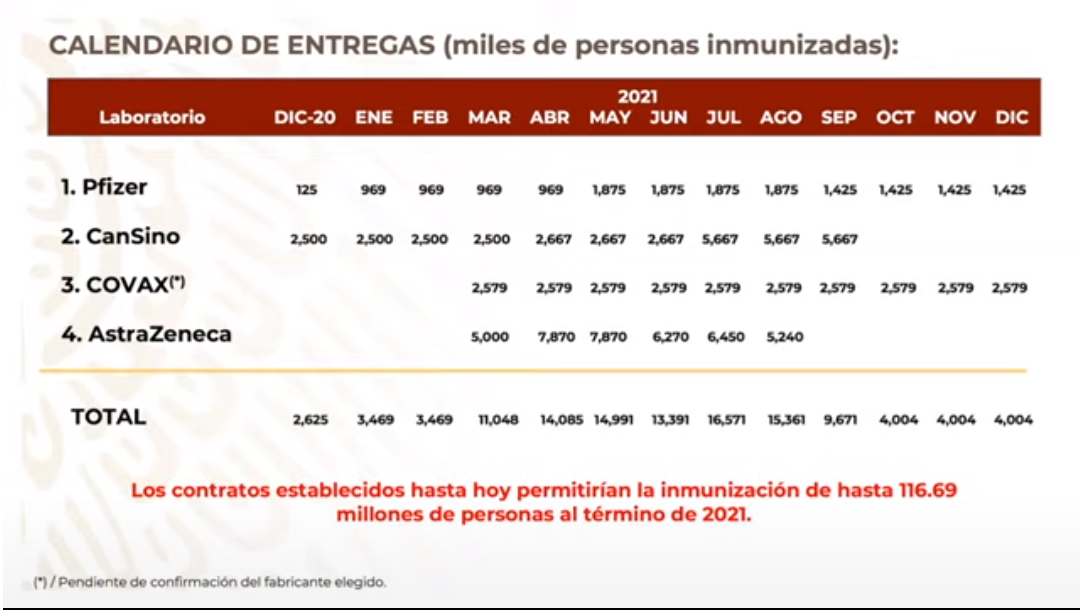
\includegraphics[%
                    width=\textwidth,
                    keepaspectratio=true]{screenshot.png}
            \end{center}
        %\end{bluebox}
        }
    \end{textblock*}
 \end{frame}


